\documentclass[10pt,a4paper]{article}
\usepackage[latin1]{inputenc}
\usepackage{amsmath}
\usepackage{amsfonts}
\usepackage{amssymb}
\usepackage{graphicx}


\usepackage{hyperref}

%%% formatting the code
\usepackage{listings}



\usepackage{color}
\lstset{%
	escapeinside={(*}{*)},%
}

\newcommand{\amidstversion}{\input{../../version.txt}}

\lstset{
	frameround=fttt,
%	language=java,
	numbers=left,
	breaklines=true,
	mathescape, 
	columns=fullflexible, 
	basicstyle=\fontfamily{lmvtt}\selectfont,
	keywordstyle=\color{blue}\fontfamily{lmvtt}\selectfont, 
	numberstyle=\color{black}
}
\lstMakeShortInline[columns=fixed]|



\newcommand{\includejavasource}[1]{\lstinputlisting[language=java]{#1}}
\newcommand{\inlinejava}[1]{\lstinline[columns=fixed,language=java]{#1}}

\newcommand{\lang}[1]{}


\begin{document}
	
	\section{About AMIDST}
	
	
	\subsection{What is AMIDST?}

AMIDST is an open source Java toolbox for scalable probabilistic machine learning with a special focus on (massive) streaming data. The toolbox allows  specifying  probabilistic graphical models with latent variables and temporal dependencies. 

For start using AMIDST, just visit the \href{getting-started.html}{Getting-started} section.

The main features of the tooblox are listed below: 
	
	\begin{itemize}
\item\textbf{ Probabilistic Graphical Models}: Specify your model using probabilistic graphical models with latent variables and temporal dependencies. AMIDST contains a large list of predefined latent variable models:


\item \textbf{Scalable inference}: Perform inference on your probabilistic models with powerful approximate and scalable algorithms.

\item \textbf{Data Streams}: Update your models when new data is available. This makes our toolbox appropriate for learning from (massive) data streams.

\item \textbf{Large-scale Data}: Use your defined models to process massive data sets in a distributed computer cluster using Apache Flink or (soon) Apache Spark.

\item \textbf{Extensible}: Code your models or algorithms within AMiDST and expand the toolbox functionalities. Flexible toolbox for researchers performing their experimentation in machine learning.

\item \textbf{Interoperability}: Leverage existing functionalities and algorithms by interfacing to other software tools such as Hugin, MOA, Weka, R, etc.
	\end{itemize}


\subsection{Scalability}
\subsubsection{Multi-Core Scalablity using Java 8 Streams}
Scalability is a main concern for the AMIDST toolbox. Java 8 streams are used to provide parallel implementations of our learning algorithms. If more computation capacity is needed to process data, AMIDST users can also use more CPU cores. As an example, the following figure shows how the data processing capacity of our toolbox increases given the number of CPU cores when learning an a probabilistic model (including a class variable C, two latent variables (LM, LG), multinomial (M1,...,M50) and Gaussian (G1,...,G50) observable variables) using the AMIDST's learning engine. As can be seen, using our variational learning engine, AMIDST toolbox is able to process data in the order of gigabytes (GB) per hour depending on the number of available CPU cores with large and complex PGMs with latent variables. Note that, these experiments were carried out on a Ubuntu Linux server with a x86\_64 architecture and 32 cores. The size of the processed data set was measured according to the Weka's ARFF format.


\begin{figure}[h!]
	\centering
	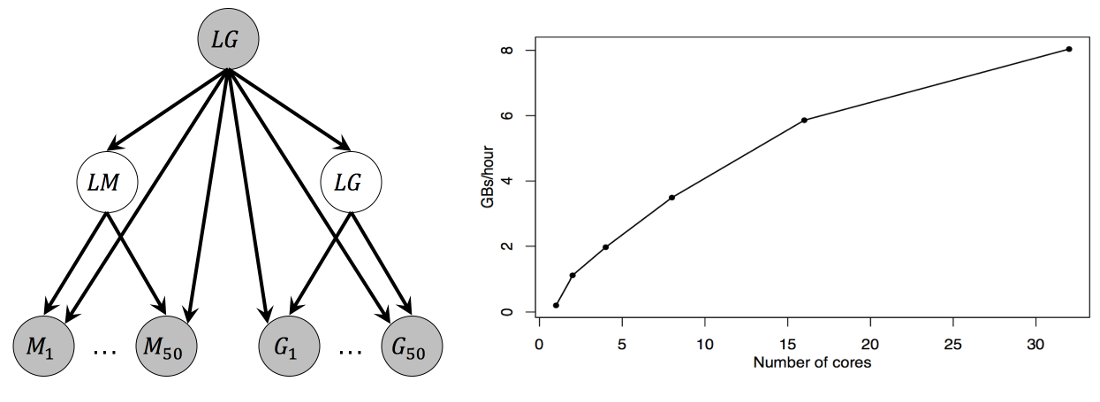
\includegraphics[width=15cm]{img/multicore_res.png}
	\caption{fig:multicoreres}
\end{figure}


\subsubsection{Distributed Scalablity using Apache Flink}
If your data is really big and can not be stored in a single laptop, you can also learn your probabilistic model on it by using the AMIDST distributed learning engine based on a novel and state-of-the-art distributed message passing scheme implemented on top of Apache Flink. we were able to perform inference in a billion node (i.e. $10^9$) probabilistic model in an Amazon's cluster with 2, 4, 8 and 16 nodes, each node containing 8 processing units. The following figure shows the scalability of our approach under these settings.



\begin{figure}[h!]
	\centering
	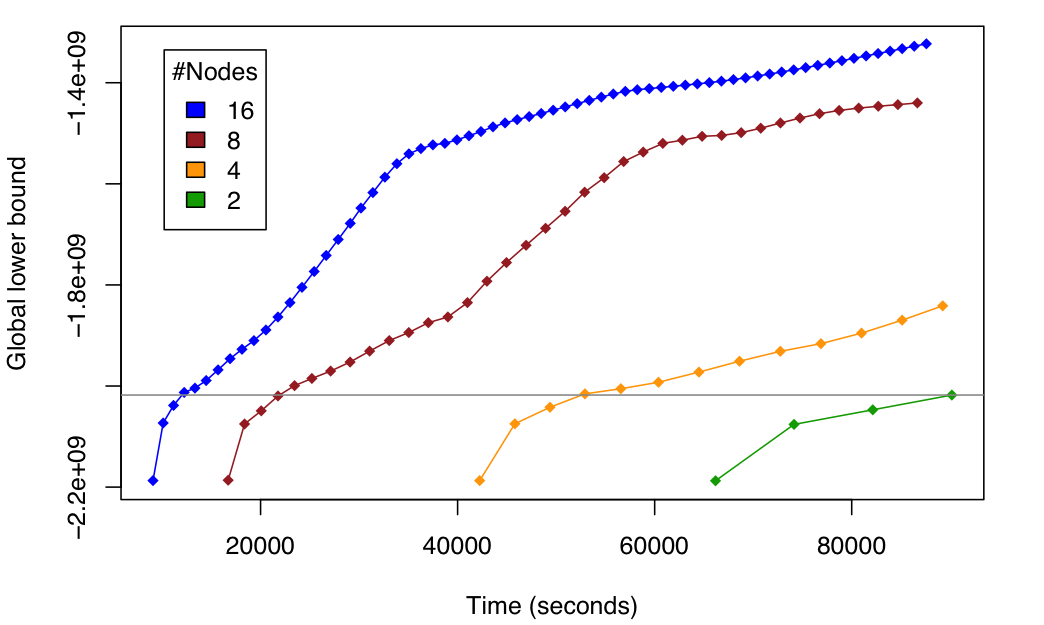
\includegraphics[width=15cm]{img/cluster_res.png}
		\caption{fig:clusterres}
\end{figure}


	\subsection{Related Software}
	
	

Numerous tools for graphical models have been published during the last three decades. See this \href{http://www.cs.ubc.ca/~murphyk/Software/bnsoft.html}{link} for an updated list. In the following table, the main features of the AMIDST toolbox are compared against other related tools.




\begin{figure}[h!]
	\centering
	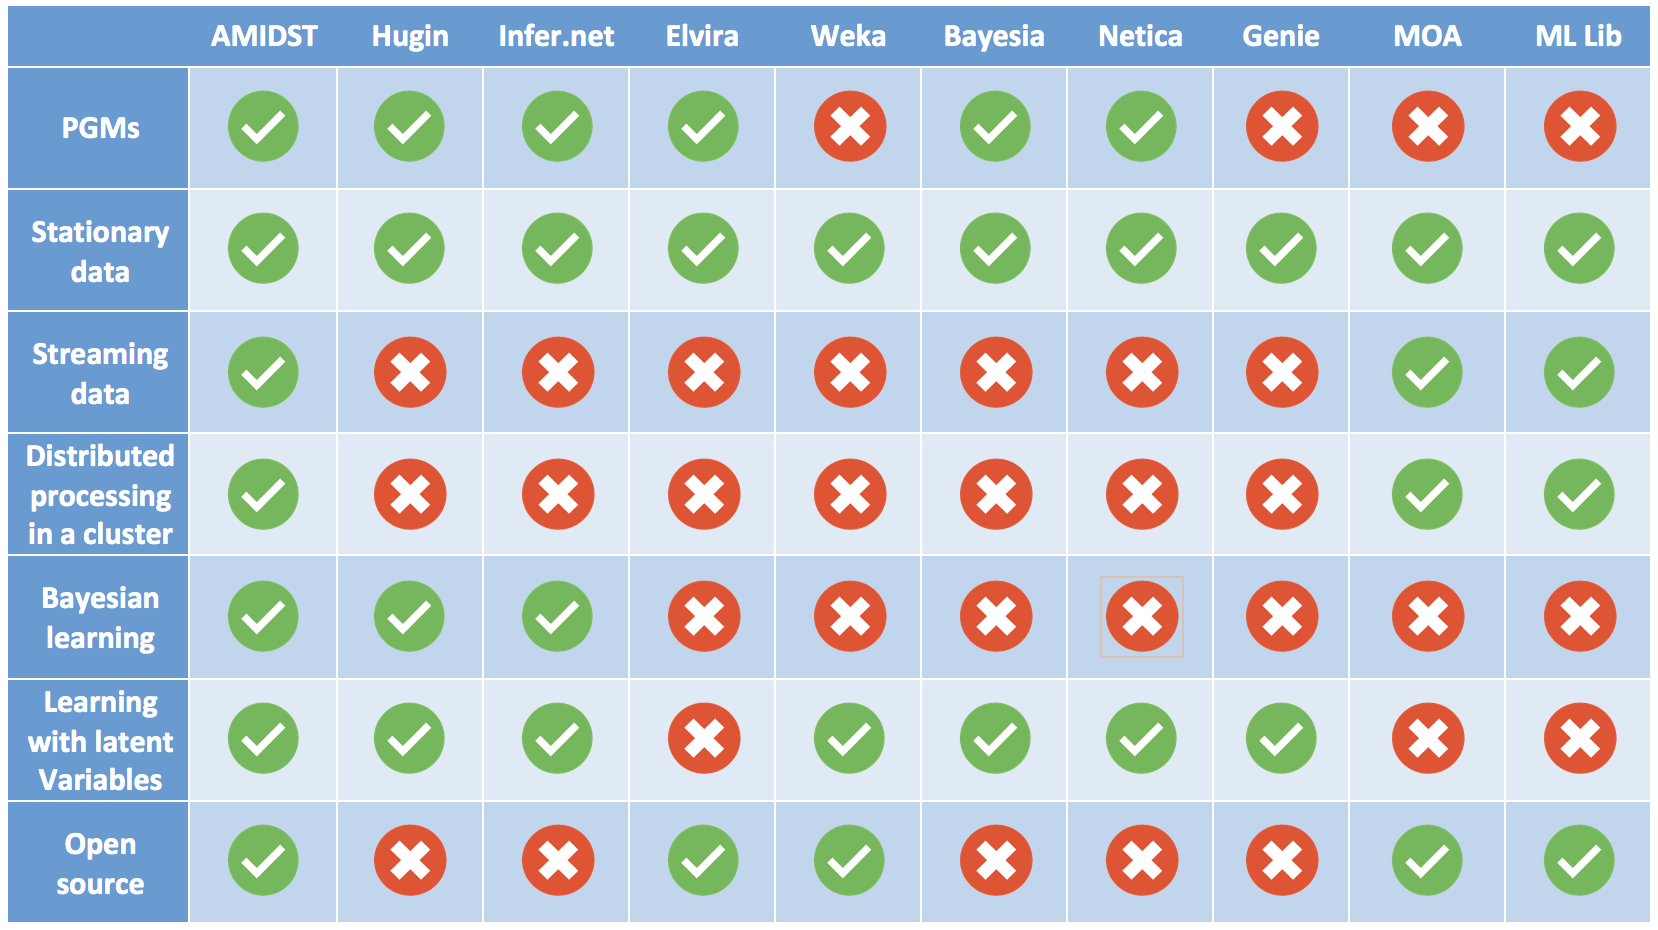
\includegraphics[width=15cm]{img/related_tools.png}
		\caption{fig:relatedtools}
\end{figure}



The vast majority of the similar tools do not support scalable inference and learning algorithms. To the best of our knowledge, this is the first PGM based software tool which is able to learn general  Bayesian networks 
from streaming data:  the rest of existing software for learning PGMs tools focus on stationary data sets. Moreover, AMIDST is able to exploit modern computing distributed processing tools like Apache Flink and Apache Spark. In the era of Big Data, this is a relevant and worthy feature. Even though MOA and ML Lib can process data streams in a distributed way, these tools do not allow learning PGMs.  \newline 




On the other hand, most of these toolboxes only deal with discrete-multinomial variables, and only few of them also support Gaussian and conditional lineal Gaussian random variables such as Hugin. However, {AMIDST} Toolbox can deal with general conjugate exponential Bayesian networks. In the current version, we support multinomial, Gaussian, Dirichlet, and  Gamma distributed random variables, and the implemented Bayesian learning algorithms are general enough to accommodate any other distribution belonging to the conjugate exponential family. Infer.net can deal with distributions in this family, however this tool is a proprietary non-portable software which cannot be run in a cluster.\newline 











\end{document}